\section{Chapter 2: Used Materials and its Features} 
In our project we have used some specific Materials … in this chapter we will discuss these Materials and its feature. Our project consists of main components including RaspberryPi, H-bridge and Wild Thumper.

\subsection{ RaspberryPi  }
The Raspberry Pi is a single-board computer with wireless LAN and Bluetooth connectivity developed by the Raspberry Pi Foundation in the UK to promote basic computer science teaching in schools and developing countries. The original model was much more popular than anticipated, selling uses such as robotics outside of its target market. This is now commonly used also in research projects, because of its low cost and portability, for example for weather monitoring. It does not contain peripherals (such as mice and keyboards), or cases. However, some official and unofficial packages included several accessories. The Raspberry Pi used in our project is the Raspberry Pi 3 which is the third and most recent Raspberry Pi generation. Just since February 2016, it replaced the Raspberry Pi 2 Model B.

\begin{figure}[ht]
    \centering
    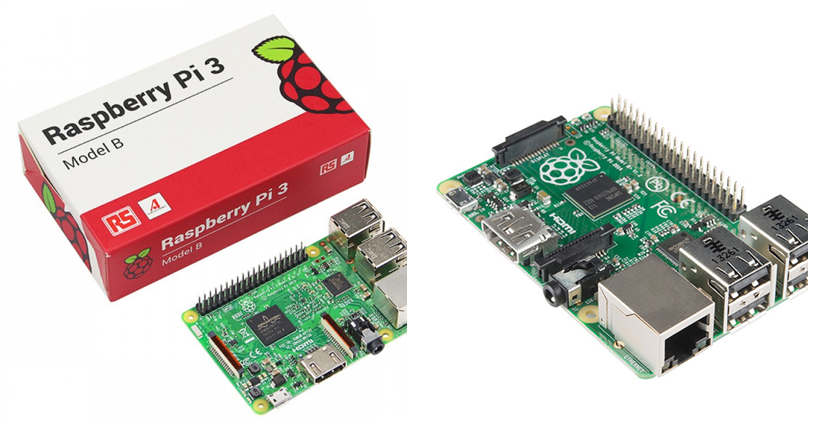
\includegraphics[width=1\textwidth]{figures/Raspberry Pi 3.png}
    \caption{Raspberry Pi 3}
\end{figure}

\section*{Features: }
\begin{itemize}
\item Quad Core 1.2GHz Broadcom BCM2837 64bit CPU.
\item 1GB RAM
\item BCM43438 wireless LAN and Bluetooth Low Energy (BLE) on board
\item 100 Base Ethernet
\item 40-pin extended GPIO
\item 4 USB 2 ports
\item 4 Pole stereo output and composite video port
\item Full size HDMI
\item CSI camera port for connecting a Raspberry Pi camera
\item DSI display port for connecting a Raspberry Pi touchscreen display
\item Micro SD port for loading your operating system and storing data
\item Upgraded switched Micro USB power source up to 2.5A
\end{itemize}

\section*{GPIO: }
An important feature of the Raspberry Pi is the row of GPIO (general input / output) pins along the board's top edge. Both existing Raspberry Pi boards (unpopulated on Pi Zero and Pi Zero W) have a 40-pin GPIO header. Until the Pi 1 Model B+ (2014) the boards had a shorter header of 26-pin.

\begin{figure}[ht]
    \centering
    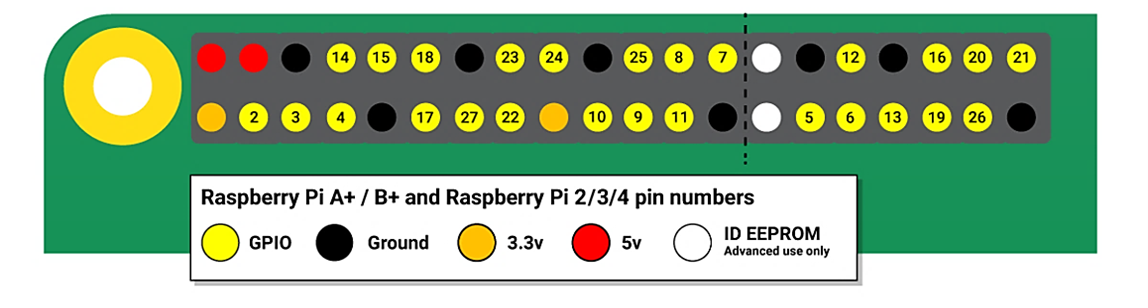
\includegraphics[width=0.8\textwidth]{figures/Raspberry Pi Pin Numbers.png}
    \caption{Raspberry Pi Pin Numbers}
\end{figure}

Any of the GPIO pins can be designated as an input or output pin (in software) and used for a broad range of purposes. Note that GPIO pins are not numbered in numerical order; GPIO pins 0 and 1 are on the board (physical pins 27 and 28), but are reserved for advanced use.

\begin{figure}[ht]
    \centering
    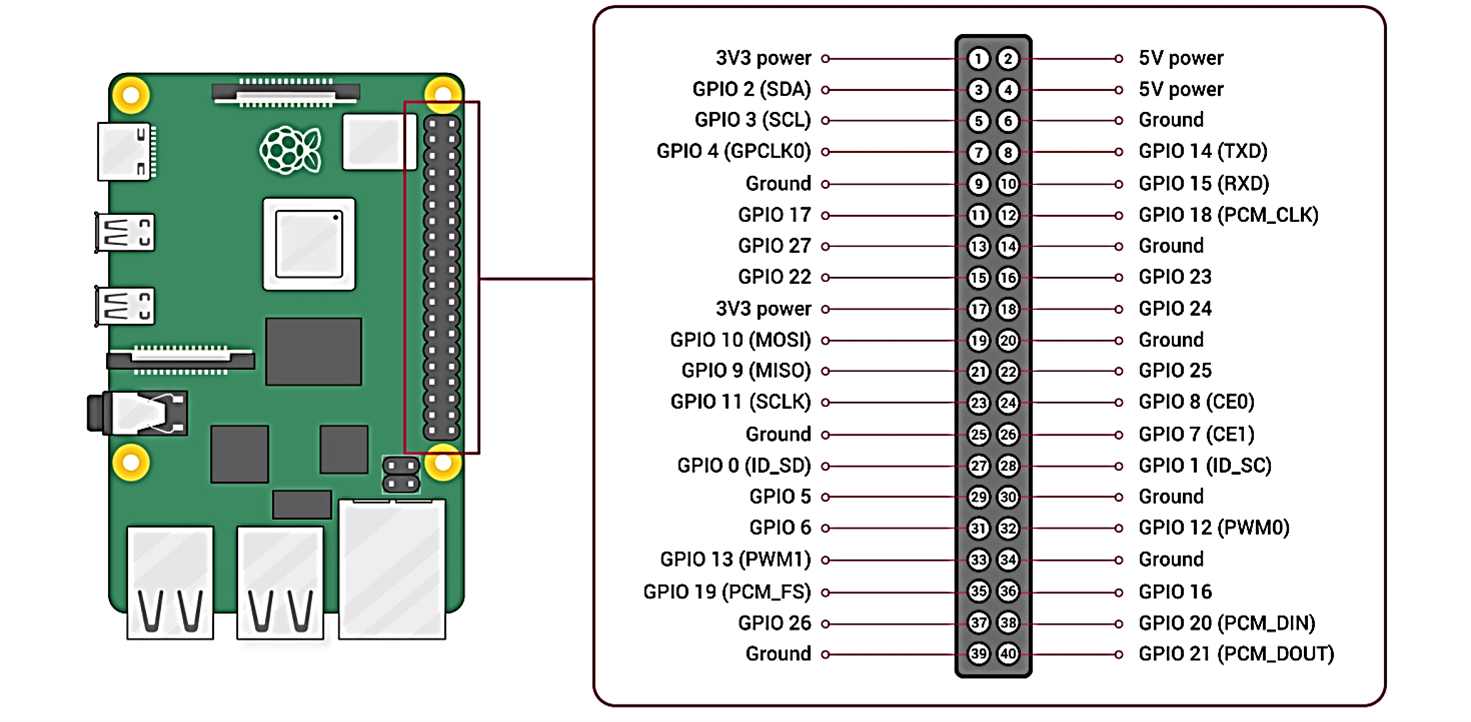
\includegraphics[width=1.2\textwidth]{figures/Raspberry Pi Pin Assignment.png}
    \caption{Raspberry Pi Pin Numbers}
\end{figure}

\section*{Voltages: }
On the board are two 5V pins and two 3V3 pins, as well as several ground pins (0V), which are unconfigurable. The remaining pins are all 3V3 pins with general purpose, meaning outputs are set to 3V3, and inputs are sensitive to 3V3.

\section*{Outputs: }
They can be set to high (3V3) or low (0V) with a GPIO pin designated as an output pin.

\section*{Inputs: }
A high (3V3) or low (0V) GPIO pin designated as an input pin may be read. This is made easier using internal pull-up resistors or pull-down resistors. GPIO2 and GPIO3 pins have fixed pull-up resistors but this can be configured in software for other pins.

\section*{More about GPIO: }
The GPIO pins can be used with a number of alternative functions as well as simple input and output devices; some are available on all pins, others on different pins.

\begin{itemize}
    \item PWM (Pulse-Width Modulation)
       \begin{itemize}
         \item Software PWM available on all pins
         \item Hardware PWM available on GPIO12, GPIO13, GPIO18, GPIO19
    \end{itemize}
    \item SPI
       \begin{itemize}
         \item SPI0: MOSI (GPIO10)
         \item MISO (GPIO9)
         \item SCLK (GPIO11)
         \item SPI1: MOSI (GPIO20)
         \item MISO (GPIO19)
         \item SCLK (GPIO21)
    \end{itemize}
    \item I2C 
       \begin{itemize}
         \item Data: (GPIO2)
         \item Clock (GPIO3)
         \item EEPROM Data: (GPIO0)
         \item EEPROM Clock (GPIO1)
    \end{itemize}
    \item Serial 
       \begin{itemize}
         \item TX (GPIO14)
         \item RX (GPIO15)
    \end{itemize}
\end{itemize}

\section*{GPIO pinout }
It's important that you know which pin is which. Some people use pin labels (such as the RasPiO Portsplus PCB, or the Raspberry Leaf printable). On the Raspberry Pi a handy reference can be accessed by opening a terminal window and running the pinout command. The GPIO Zero Python library provides this tool, which is installed by default on the Raspberry Pi OS desktop image but not on Raspberry Pi OS Lite.

\subsection{ H-bridge  }
An H-bridge is an electronic circuit that switches the polarity of a voltage applied to a load. These circuits are often used in robotics and other applications to allow DC motors to run forwards or backwards. 
The H-bridge used in our project is (BTS7960B H-bridge 43A) high-power motor driver Module (For Single Motor). This driver uses Infineon chips BTS7960 composed of high-power drive full H-bridge driver module with thermal over-current protection. Double BTS7960 H-bridge driver circuit, with a strong drive and braking, effectively isolating the microcontroller and motor driver! High-current 43A

\begin{figure}[ht]
    \centering
    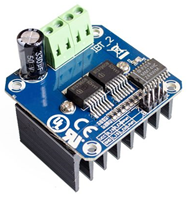
\includegraphics[width=0.4\textwidth]{figures/BTS7960B H-bridge.png}
    \caption{Raspberry Pi Pin Numbers}
\end{figure}

\section*{ Features: }
\begin{itemize}
    \item Double BTS7960 large current (43 A) H bridge driver.
    \item 5V isolate with MCU, and effectively protect MCU.
    \item 5V power indicator on board.
    \item Input supply voltage 5.5V to 27V.
    \item Voltage indication of motor driver output end.
    \item Just need four lines from MCU to driver module (GND. 5V. PWM1. PWM2).
    \item Able to reverse the motor forward, two PWM input frequency up to 25 kHz.
    \item Two heat flow passing through an error signal output.
    \item Isolated chip 5V power supply (can be shared with the MCU 5V), can also use the on-board 5V supply.
\end{itemize}

\section*{ Wild Thumper }
The robust “Wild Thumper” 6WD All Terrain Chassis for robotic applications is made from 2mm thick anodized aluminum plates with stainless steel and nickel plated brass fittings. Custom electronic boards and sensors can be mounted easily on the many 4mm holes which are arranged in a 10mm grid. The Wild Thumper is equipped with 6 powerful steel gearbox motors (1:35 ratio, 4kg/cm stall torque per Motor), spiked tractor tires and a “Super Twist” suspension system to keep all wheels on the ground. This chassis will let your robot go almost anywhere in rough terrain and drive over obstacles. The platform is perfect for robotic developers and student projects. Between the wheels are two large Battery compartments which can hold up to 4 x 7, 2 V RC Car subs C Battery Packs.

\begin{figure}[h]
    \centering
    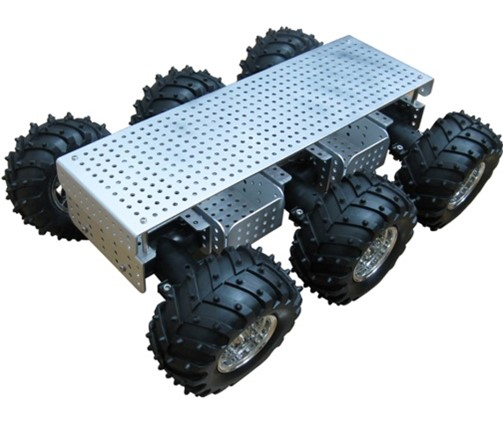
\includegraphics[width=0.4\textwidth]{figures/Wild Thumper.jpg}
    \caption{Raspberry Pi Pin Numbers}
\end{figure}

\section*{ Specifications: }
\begin{itemize}
    \item Dimensions: (L x W x H) 430 x 310 x 135 mm.
    \item 2mm thick anodized aluminum plates.
    \item Adjustable “Supertwist” suspension system.
    \item 6 spiked tractor tires.
    \item Rotation speed: 295 rpm.
\end{itemize}

